\documentclass[10pt,a4paper]{article}
\usepackage[english,polish]{babel}
\usepackage[utf8]{inputenc}
\usepackage{polski}
\usepackage{indentfirst}
\usepackage{mathtools} 
\usepackage[a4paper,margin=2cm]{geometry}
\usepackage{tabularx}
\usepackage{graphicx}
\usepackage{float}

\usepackage[hidelinks]{hyperref}

\usepackage{amsmath}
\usepackage{algorithm}
\usepackage[noend]{algpseudocode}

\usepackage{listings}
\lstloadlanguages{TeX}
\lstset{
  literate={ą}{{\k{a}}}1
           {ć}{{\'c}}1
           {ę}{{\k{e}}}1
           {ó}{{\'o}}1
           {ń}{{\'n}}1
           {ł}{{\l{}}}1
           {ś}{{\'s}}1
           {ź}{{\'z}}1
           {ż}{{\.z}}1
           {Ą}{{\k{A}}}1
           {Ć}{{\'C}}1
           {Ę}{{\k{E}}}1
           {Ó}{{\'O}}1
           {Ń}{{\'N}}1
           {Ł}{{\L{}}}1
           {Ś}{{\'S}}1
           {Ź}{{\'Z}}1
           {Ż}{{\.Z}}1,
  basicstyle=\footnotesize\ttfamily,
}

\frenchspacing
\usepackage{tabto}

\usepackage{titlesec}
\titlelabel{\thetitle.\quad}

\begin{document}
	\title{PSRA - raport  \\  Algorytm Flux Tensor with Split Gaussian models}
	\author{Piotr Janus, Kamil Piszczek}
	\date{}
	\maketitle


\section{Wprowadzenie}

Opracowanie i implementacja sprzętowa algorytmu \textit{FTSG}, było głównym celem przedstawianego projektu. Algorytm ten jest metodą hybrydową, dzięki czemu posiada wszystkie zalety algorytmów \textit{Flux Tensor} (rozdział \ref{sec:FluxTensor_Teoria}) oraz \textit{Split Gaussian Models} (rozdział \ref{sec:split_gaussian}).   

Obie wykorzystywane metody nie są idealne, jednak wzajemnie się uzupełniają przez co można opracować algorytm wykorzystujący je jednocześnie. Metoda \textit{Flux Tensor} nie daje możliwości wykrywania obiektów statycznych. Zapewnia jednak odporność na zakłócenia spowodowane zmianami oświetlenia, a częściowo także przez występowanie cieni. Przeciwieństwem jest algorytm wykorzystujący rozkłady Gaussa, o ograniczonej odporności na zakłócenia, ale dający możliwość wykrywania obiektów statycznych. 

\section{Metoda Flux Tensor}
\label{sec:FluxTensor_Teoria}

\subsection{Opis Algorytmu}
\label{sec:FluxTensorOpis}

Algorytm \textit{Flux Tensor} jest uniwersalną metodą wykrywania ruchomych obiektów na obrazie ze statycznej kamery. Metoda ta jest niewrażliwa na zmiany oświetlenia, jednak przy jej użyciu nie jesteśmy w stanie rozpoznać statycznych obiektów pierwszoplanowych. Algorytm opiera się na detekcji krawędzi poziomych i pionowych, a następnie obliczeniu pochodnej obrazu po czasie, w celu wykrycia ruchomych elementów.

Metoda \emph{Flux Tensor} w przedstawionej wersji operuje na obrazie w skali szarości. Oznaczmy przez $I(x,y,t)$ wartość piksela wejściowego. Gdzie $x,y$ to współrzędne piksela na obrazie, $t$ – czas. Dla uproszczenia wektor w przestrzeni $(x,y,t)$ możemy zapisać jako $v$.
\textit{Flux Tensor} możemy przedstawić, jako macierz, opisującą zmiany wartości piksela wejściowego w lokalnej trójwymiarowej czasoprzestrzeni. Przez $\Omega$ rozumiemy otoczenie w przestrzeni $(x,y,t)$, które rozważamy przy analizie danego piksela. Zgodnie z artykułem \cite{wang_14} macierz Flux Tensor wygląda następująco:
 
\begin{equation}
			J_F(i) = 
			\begin{pmatrix}
			\int_\Omega \left(\frac{\partial^2 I(v)}{\partial x\partial t}\right)^2\,dv & 
			\int_\Omega \frac{\partial^2 I(v)}{\partial x\partial t}\frac{\partial^2 I(v)}{\partial y 							\partial t}\,dv & 
			\int_\Omega \frac{\partial^2 I(v)}{\partial x\partial t}\frac{\partial^2 I(v)}{\partial^2 t}						\,dv	\\
			
			\int_\Omega \frac{\partial^2 I(v)}{\partial y\partial t}\frac{\partial^2 I(v)}{\partial x 							\partial t}\,dv & 
			\int_\Omega \left(\frac{\partial^2 I(v)}{\partial y\partial t}\right)^2\,dv & 
			\int_\Omega \frac{\partial^2 I(v)}{\partial y\partial t}\frac{\partial^2 I(v)}{\partial^2 t}						\,dv \\
			
			\int_\Omega \frac{\partial^2 I(v)}{\partial^2 t}\frac{\partial^2 I(v)}{\partial x\partial t}						\,dv & 
			\int_\Omega \frac{\partial^2 I(v)}{\partial^2 t}\frac{\partial^2 I(v)}{\partial y\partial t}						\,dv & 
			\int_\Omega \left(\frac{\partial^2 I(v)}{\partial^2 t}\right)^2\,dv \\		
			\end{pmatrix}
\label{equ:fluxTensorMatrix}
\end{equation}

Elementy macierzy zawierają informację na temat zmiany gradientu w czasie, co pozwala na rozróżnienie elementów ruchomych i statycznych na obrazie. Detekcja odbywa się bezpośrednio na podstawie śladu macierzy: 

\begin{equation}
	trace(J_F) = \int_\Omega \left\lVert \frac{\partial}{\partial t}\nabla I(v) \right\rVert^2\,dv
\label{equ:fluxTrace}
\end{equation}

Ślad macierzy jest obliczany dla każdego piksela. Jeżeli jego wartość jest większa od ustalonej wartości progowej $T$, to analizowany piksel jest elementem ruchomego obiektu. W przeciwnym wypadku zakładamy, że piksel jest tłem.
Przyjmijmy następujące oznaczenia:

\begin{equation}
	I_{xt}=\frac{\partial^2I(x,y,t)}{\partial x\partial t},\quad I_{yt}=\frac{\partial^2I(x,y,t)}{\partial y			\partial t},\quad I_{tt}=\frac{\partial^2I(x,y,t)}{\partial^2 t}	
\label{equ:fluxComponents}
\end{equation}

Równanie (\ref{equ:fluxTrace}) można wówczas zapisać jako:

\begin{equation}
	trace(J_F) = \int_\Omega \left(I_{xt}^2(i) + I_{yt}^2(i) + I_{tt}^2(i)\right)\,dv
\label{equ:fluxTraceFinal}
\end{equation}

Składowe $I_{xt}$ i $I_{yt}$ zawierają informację o wykrytych i jednocześnie poruszających się krawędziach (na podstawie pochodnej po czasie), natomiast $I_{tt}$ informuje o zmianach oświetlenia w czasie.
	
\subsection{Obliczenia numeryczne}
\label{sec:FluxObliczenia}

W pierwszym kroku piksel w formacie $\small{RGB}$ konwertowany jest do skali szarości zgodnie z zależnością:

\begin{equation}
GRAY = 0.21R + 0.72G + 0.07B
\label{equ:grayscaleConversion}
\end{equation}

Składowe $I_{xt}$, $I_{yt}$, $I_{tt}$ są obliczane z wykorzystaniem jednowymiarowych masek konwolucji. Jest to rozwiązanie mniej złożone obliczeniowo, niż stosowanie masek 3D. Dodatkowo, w~celu redukcji szumów, używany jest jednowymiarowy filtr wygładzający dla składowej, która nie występuje w~aktualnie obliczanej pochodnej.
 
Zgodnie z powyższym, podczas obliczania składowej $I_{xt}$ są używane filtry różniczkujące dla składowych $x$ i $t$, oraz filtr wygładzający dla składowej $y$. Analogicznie, w przypadku składowej $I_{yt}$ należy wykorzystać filtr wygładzający dla składowej $x$. Ostatnim elementem jest składowa $I_{tt}$. Tutaj filtry wygładzające używane są dla składowych $x$ i $y$. Operacja całkowania jest wykonywana z~użyciem odpowiednich jednowymiarowych filtrów. Na obraz nakładane są maski uśredniające dla poszczególnych składowych. Schemat tych operacji został przedstawiony na rys. \ref{fig:FluxOperationFlow}.

		\begin{figure}[h!]
				\centering
				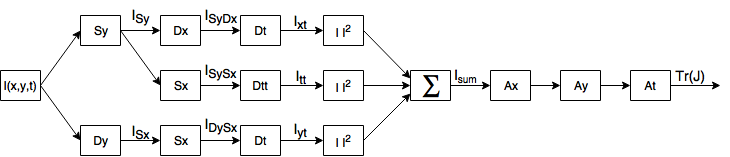
\includegraphics[scale=0.6]{img/FluxOperationFlow.png}
				\caption{Schemat operacji wyznaczających ślad macierzy $J_F$}
				\label{fig:FluxOperationFlow}
		\end{figure}

\noindent Przedstawione na rys. \ref{fig:FluxOperationFlow} operacje to odpowiednio: \\
\hspace*{1cm}	$Dx$,\  $Dy$ -- filtry różniczkujące odpowiednio dla składowych $x$ i $y$\\
\hspace*{1cm}	$Sx$,\  $Sy$ -- filtry wygładzające dla składowych $x$ i $y$\\
\hspace*{1cm}	$Dt$,\  $Dtt$ -- odpowiednio pierwsza i druga pochodna z wartości piksela po czasie\\
\hspace*{1cm}	$Ax$,\  $Ay$ -- filtry uśredniające przestrzenne\\
\hspace*{1cm}	$At$ -- filtr uśredniający czasowy\\

Oprócz rozmiarów poszczególnych filtrów algorytm posiada także parametr $T$, czyli próg wartości śladu, macierzy, powyżej którego piksel zostaje uznany za tło. Ostateczna lista parametrów algorytmu wygląda następująco:\\
\-\hspace{1cm} $T$ --wartość progowa\\
\-\hspace{1cm}	$nDs$ -- rozmiar filtrów przestrzennych (różniczkujących i wygładzających)\\
\-\hspace{1cm}	$nDt$ --  liczba ramek używana do różniczkowania po czasie\\
\-\hspace{1cm}	$nAs$ -- rozmiar masek uśredniających przestrzennych\\
\-\hspace{1cm}	$nAt$ -- liczba ramek używana do uśredniania po czasie\\

Należy zwrócić uwagę, że dobranie dużych rozmiarów filtrów (szczególnie różniczkujących po czasie) znacząco zwiększa zużycie pamięci.
Domyślnymi parametrami, sprawdzającymi się w~większości przypadków są: 
\begin{center}
$T = 25$, \quad $nDs = 5$, \quad $nDt = 5$, \quad $nAs = 5$, \quad $nAt = 5$
\end{center}
Jak wcześniej wspomniano, schemat na rys. \ref{fig:FluxOperationFlow}, zoptymalizowany został pod kątem zużycia pamięci z~zachowaniem równoległości obliczeń. W tym przypadku do działania algorytmu będą potrzebne 3 bufory o rozmiarze $nDt-1$ każdy oraz jeden bufor o rozmiarze $nAt-1$. Bufory działają na zasadzie kolejki \textit{FIFO} (ang. \textit{First In, First Out} -- pierwszy na wejściu, pierwszy na wyjściu). W przypadku domyślnych parametrów wiąże się to z~przechowywaniem w pamięci 16 ramek obrazu.

\subsection{Implementacja sprzętowa}

Wstępna analiza algorytmu przedstawionego na rysunku \ref{fig:FluxOperationFlow} pozwoliła wskazać dwa podstawowe wyzwania związane z realizacją sprzętową.
Po pierwsze, z uwagi na konieczność buforowania 16 ramek obrazu (domyślne parametry) niezbędne okazało się być użycie zewnętrznej pamięci RAM -- współcześnie dostępne układy FPGA nie posiadają wystarczających zasobów pamięciowych do buforowania ramek HD. Po drugie algorytm wymaga wykonania wielu operacji kontekstowych. W celu zaoszczędzenia zasobów, warto ustawić operacje w takiej kolejności, aby pierwsze wykonywane były operacje wykorzystujące kontekst pionowy.

Jak zaznaczono wcześniej, wyliczanie różniczki i uśrednianie po czasie (operacje $D_t, D_{tt}, A_t$ ) wymagają buforowania poprzednich ramek --  wartości $I_{S_yD_x}$, $I_{S_yS_x}$, $I_{D_yS_x}$ oraz $I_{sum}$. 
Liczba zapamiętywanych wartości zależy od zastosowanych rozmiarów masek. 
Dla podanych wcześniej parametrów (wszystkie maski o~rozmiarze 5), dla pojedynczego piksela wymaga się $(5-1)*4*8$ bitów $= 128$ bitów.
Dla maksymalnego rozważanego rozmiaru maski $n=7$ wskaźnik ten wynosi $192$ bity.
Wyznaczone wartości nie przekraczają możliwości współczesnych układów FPGA współpracujących z szybkimi pamięciami DDR3 lub DDR4, nawet dla rozdzielczości HD.

\subsubsection{Stworzona architektura}

Ogólny schemat zrealizowanego modułu sprzętowego przedstawiono na rysunku \ref{fig:jpk_FluxMainFlow}.
Wszystkie moduły zostały opisane w języku Verilog, w trakcie prac wykorzystywano środowisko Vivado w wersji 2015.4 firmy Xilinx.

\begin{figure}[h!]
	\centering
	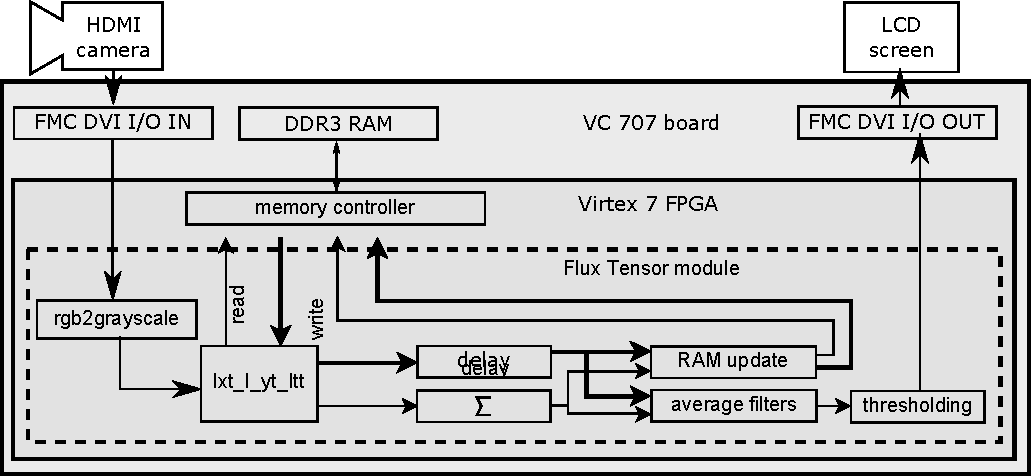
\includegraphics[width=12cm]{img/flux_architecture.pdf}
	\caption{Architektura zaimplementowana w układzie FPGA}
	\label{fig:jpk_FluxMainFlow}
\end{figure}

Źródłem sygnału wizyjnego była kamera Sony HDR-CX280 z wyjściem HDMI.
Do wizualizacji rezultatów działania systemu wykorzystano typowy monitor LCD z wejściem HDMI.
Wszystkie obliczenia realizowane byłby na karcie ewaluacyjnej VC 707 firmy Xilinx.
Centralnym elementem platformy jest układ FPGA Virtex 7 (XC7VX485T–2FFG1761).
W rozwiązaniu wykorzystano ponadto zewnętrzną pamięć DDR3 RAM oraz moduł wejścia/wyjścia  HDMI (przystawka Avnet FMC DVI I/O).

W pierwszym kroku sygnał wejściowy konwertowany jest z przestrzeni barw RGB do skali szarości (moduł \texttt{rgb2grayscale}).
Zastosowano przekształcenie zgodne z~biblioteką OpenCV.

W następnym module wyznaczane są składowe $I_{xt}, I_{yt}, I_{tt}$ (szczegółowy opis modułu w Subsection \ref{ssec:trace_computation}).
Obliczanie pochodnych po czasie wymaga wykorzystania kontrolera pamięci (moduł \texttt{memory controller}).
Następnie wyliczane wartości są podnoszone do kwadratu oraz sumowane (moduł $\Sigma$).
Równolegle następuje opóźnienie danych odczytanych z pamięci RAM.

Wyniki poprzednich operacji trafiają do dwóch modułów:
\begin{itemize}
\item \texttt{RAM update} -- następuje tutaj aktualizacja danych, które mają zostać zapisane do pamięci RAM. Polega ona na operacji FIFO (First In First Out) tj. usunięciu najstarszego elementu z wektora danych, %przesunięcia pozostałych danych oraz dodania nowego elementu.
\item  \texttt{avarage filters} -- realizacja uśredniania (filtry $A_x, A_y, A_t$) -- omówienie w Subsection \ref{ssec:spatial_averaging}.
\end{itemize}
Ostatnim etapem algorytmu jest binaryzacja (moduł \texttt{thersholding}.

W trakcie projektowania modułu dążono do redukcji zasobów poprzez ograniczenie długości linii opóźniających dla dany zapisanych w pamięci RAM (słowo o szerokości 128 bitów).
Po pierwsze dane czytano dokładnie w momencie, kiedy były potrzebne.
Ponadto zdecydowano się na zapisanie do pamięci wartości $I_{sum}$, nie $I_{sum}$ po operacjach $A_x$ i $A_y$.
Zastosowanie takiego podejścia wiąże się z koniecznością realizacji filtracji $A_x$ i $A_y$ dla wszystkich pikseli z kontekstu czasowego (tj. $5$ w rozważanym przypadku).
Jeśli weźmie się pod uwagę tylko długie linie opóźniające (zrealizowane w pamięci BRAM), to przy takim rozwiązaniu niezbędne jest pamiętanie: $YY \cdot 4 \cdot 5 \cdot 8 = 160 \cdot XX $ bitów (YY -- rozdzielczość %pozioma obrazów).
Alternatywne rozwiązanie, tj. bezpośrednia realizacja wg. schematu z rysunku \ref{fig:FluxOperationFlow}, wymaga pamiętania $YY \cdot 4 \cdot 128 = 512 \cdot YY$ bitów.

Warto też zaznaczyć, że zastosowane skrócenie ścieżki może mieść również inne zalety.
Przykładowo, jeśli moduł FT wykorzysta się w ramach bardziej rozbudowanego systemu wizyjnego, to brak konieczności opóźniania pozostałych danych zapisanych w pamięci RAM jest bardzo pożądany i może pozwolić na dużo większą redukcję zapotrzebowania na zasoby.

\subsubsection{Moduł obliczający ślad macierzy}
\label{ssec:trace_computation}
Szczegółowy schemat modułu \texttt{I\_xt\_I\_ty\_I\_tt} przedstawiono na rysunku \ref{fig:FluxTraceFinal}.
Na początku wyliczany jest kontekst pionowy. W momencie gdy na wyjściu modułu pojawi się poprawny kontekst tj. wektor 5 pikseli,  generowany jest sygnał odczytu z pamięci RAM (\texttt{read}), tak aby dostępne były zapisane dla rozważanego piksela dane.
Mają one następującą postać: \\
$[I_{S_yD_x(t-1)}, ... ,I_{S_yD_x(t-nDt+1)},
I_{D_yS_x(t-1)}, ... ,I_{D_yS_x(t-nDt+1)}, \\
I_{S_yS_x(t-1)}, ... ,I_{S_yS_x(t-nDt+1)},
I_{sum(t-1)}, ... ,I_{sum(t-nAt+1)}]$

W drugim kroku, w sposób równoległy realizowane są następujące operacje filtr rożniczkujący $D_y$ oraz filtr uśredniający $S_y$. 
Następnie wykonywane są operacje $S_x$ (dwukrotnie) oraz  $D_y$.
W trzecim etapie obliczane są różniczki po czasie $D_{t}$ i $D_{tt}$.
Niezbędne dane z pamięci RAM opóźniane są w modułach $DEL\_D_yS_x$, $DEL\_S_yD_x$ oraz $DEL\_S_yS_x$.
Dodatkowo opóźniane są dane z RAM potrzebne na etapie uśredniania przestrzennego $DEL\_I_{sum}$.
Wyjściem z modułu są wartości $I_{xt}, I_{yt}, I_{yt}$ oraz dane z pamięci RAM oznaczone prefiksem~$R\_$.

\begin{figure}[h]
	\centering
	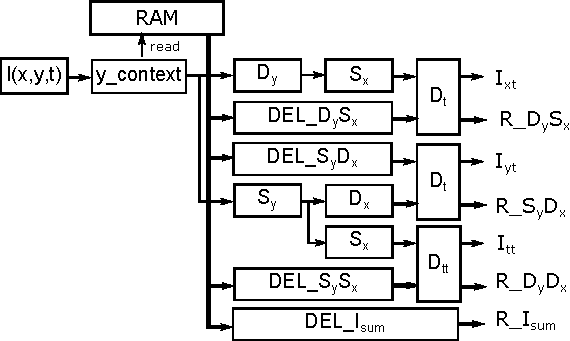
\includegraphics[width=7cm]{img/Ixt_Iyt_Itt.pdf}
	\caption{Schemat modułu obliczającego ślad macierzy (\texttt{I\_xt\_I\_ty\_I\_tt})}
	\label{fig:FluxTraceFinal}
\end{figure}

\subsubsection{Uśrednianie}
\label{ssec:spatial_averaging}

Schemat modułu \texttt{average\_filters} przedstawiono na rysunku \ref{fig:jpk_spatial_averaging}.
Wejście stanowi suma $I_{sum}$ dla bieżącej ramki oraz $nAt-1$ wartości $I_{sum}$ z poprzednich ramek (prefiks $R\_$).
W pierwszym kroku dane zostają rozdzielone na $nAt$ wartości.
Następnie dla każdej z nich wykonywane są operacje $A_x$ oraz $A_y$.
W kolejnym etapie następuje ich połączenie w temporal context dla którego wykonywana jest operacja $A_t$.
W wyniku otrzymuje się ślad macierzy $Tr(J_F)$.

\begin{figure}[h]
	\centering
	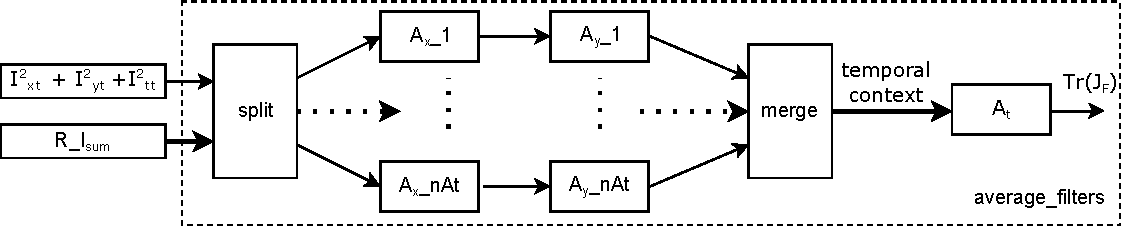
\includegraphics[width=12cm]{img/jpk_spatial_averaging.pdf}
	\caption{Moduł uśredniający $A_x, A_y, A_t$}
	\label{fig:jpk_spatial_averaging}
\end{figure}

\section{Metoda Split Gaussian Models}
\label{sec:split_gaussian}

\subsection{Opis Algorytmu}

\textit{Split Gaussian Models} jest modyfikacją metody \textit{Gaussian Mixture Models}, która jest powszechnie stosowana w systemach wizyjnych realizujących segmentację obiektów pierwszoplanowych. Działanie algorytmu jest oparte na sukcesywnie budowanym, wielowartościowym modelu tła oraz pierwszego planu. Model ten, indywidualny dla każdego piksela na obrazie, jest złożony z pewnej liczby rozkładów Gaussa. Każdy z nich charakteryzuje się wagą, średnią oraz odchyleniem standardowym. Budowany model jest więc modelem statystycznym.

W porównaniu z \textit{Gaussian Mixture Models}, którego model stanowi mieszaninę rozkładów Gaussa reprezentujących pierwszy plan oraz tło, w metodzie \textit{Split Gaussian Models} zdefiniowane są dwa odzielne modele: obiektów pierwszoplanowych oraz tła. Dodatkowo, w tym drugim modelu liczba rozkładów Gaussa zmienia się dynamicznie. Takie zmiany zapobiegają zjawisku, w którym rozkłady Gaussa reprezentujące pierwszy plan zaczynają dominować w modelu i pogarszać otrzymywane rezultaty przetwarzania. Następny akapit przedstawia szczegółowy opis algorytmu.

Wektor zawierający składowe \textit{RGB} piksela o współrzędnych $x$, $y$ w czasie $t$ oznaczmy jako $I_t(x,y)$. Następnie sprawdzamy, czy piksel pasuje do któregoś ze zdefiniowanych rozkładów Gaussa reprezentujących tło (oznaczmy liczbę takich rozkładów jako $K$). Metryka wykorzystana w teście dopasowania wygląda następująco:

\begin{equation}
D_{min}(x,y) = min_{t \in K} \: max_{j \in C} ((I_t(x,y)-\mu_{i,j})^2-T_b \cdot \sigma ^2)
\label{equ:d_min}
\end{equation}

\noindent Gdzie $\sigma = \sum_{i}^{k} \omega_i \sigma_i$. $T_b$ jest z góry ustalonym progiem (domyślnie $3$), natomiast $\mu_{i,j}$ oznacza wartość średnią dla danego rozkładu i składowej RGB. Dla uproszczenia przyjmujemy, że dla wszystkich trzech składowych odchylenie standardowe i wariancja są takie same. Piksel zostaje zaklasyfikowany jako pierwszoplanowy, jeżeli nie pasuje do żadnego z rozkładów Gaussa:

\begin{equation}
F_B(x,y) = 
\begin{cases}
1 & \quad \text{jeżeli } D_{min}(x,y)>0\\
0 & \quad \text{w przeciwnym przypadku}\\
\end{cases}
\label{equ:F_B}
\end{equation}

Model reprezentujący pierwszyplan, składający się tylko z jednego rozkładu Gaussa, jest używany do rodzielnia rzeczywistych obiektów statyczny od różnego rodzaju zakłóceń. Jeżeli piksel zostanie zaklasyfikowany jako element tła przez metodę \textit{Flux Tensor} (rozdział \ref{sec:FluxTensor_Teoria}) i jako element pierwszego planu przez model reprezentujący tło ($F_B = 1$) to ostateczna klasyfikacja (jako pierwszoplanowy element statyczny bądź zakłócenia) odbywa się z wykorzystaniem modelu pierwszego planu:

\begin{equation}
F_S(x,y) =
\begin{cases}
1 & \quad \text{jeżeli } F_{amb}(x,y)=1 \quad \text{i} \quad I_t(x,y)-\mu_f(x,y) < T_f \\
0 & \quad \text{w przeciwnym przypadku}\\
\end{cases}
\label{equ:F_S}
\end{equation}

\noindent Gdzie $F_{amb}$ określa czy wystąpiła sprzeczność w klasyfikacji pomiędzy algorytmem \textit{Flux Tensor} i modelem tła. $T_f$ jest z góry ustalonym progiem (domyślnie $20$), natomiast $\mu_f(x,y)$ aktualną wartością średnią.

\subsection{Aktualizacja rozkładów Gaussa}

Wykorzystana została tzw. konserwatywna metoda aktualizacji, polegająca na tym, że odbywa się ona tylko wtedy gdy rozpatrywany piksel pasuje do danego modelu. Model tła aktualizowany jest tylko wtedy, gdy maska $M$ zdefiniowana przez wzór \ref{equ:update_mask} ma wartość $1$, w przeciwnym wypadku aktualizowany jest jedynie model pierwszoplanowy.

\begin{equation}
M = (1-F_B) \lor (F_{amb} - F_S)
\label{equ:update_mask}
\end{equation}

\noindent Aktualizację wartości średnich i odchylenia standardowego przedstawiają odpowiednio wzory (\ref{equ:mean_update}) i (\ref{equ:sigma_update}).

\begin{equation}
\mu_t = (1-\alpha)\mu_{t-1} + \alpha I_t
\label{equ:mean_update}
\end{equation}
\begin{equation}
\sigma_t^2 = (1-\alpha) \sigma_{t-1}^2 + (I_t-\mu)^T \alpha (T_t - \mu)
\label{equ:sigma_update}
\end{equation}

\noindent W przypadku rozkładu dla którego wartość metryki, zdefiniowanej przez wzór (\ref{equ:d_min}), była najmniejsza, waga aktualizowana jest według wzoru (\ref{equ:w_update1}) w przeciwnym wypadku wykorzystywana jest zależność (\ref{equ:w_update2}).

\begin{equation}
\omega_{i,t} = (1-\alpha) \omega_{i,t-1} + \alpha
\label{equ:w_update1}
\end{equation}
\begin{equation}
\omega_{i,t} = (1-\alpha) \omega_{i,t-1}
\label{equ:w_update2}
\end{equation}

\noindent Gdzie $\alpha$ oznacza współczynnik uczenia się, domyślnie wynosi on $0.004$ dla modelu tła i $0.5$ dla modelu pierwszegoplanu.


\subsection{Architektura}

Ze względu na to, że model programowy metody \textit{Split Gaussian Models} nie dał oczekiwanych rezultatów w stosunku do wyników otrzymanych w artykule opisującym ten algorytm, implementacja sprzętowa nie została zrealizowana.

Gotowa implementacja sprzętowa metody \textit{Gaussian Mixture Models} z pewnością ułatwi w przyszłości przeniesienie na platformę FPGA naprawionego algorytmu \textit{Split Gaussian Model}. Moduł realizujący sieć sortującą, może być wykorzystany  do implementacji zmienionej metryki (\ref{equ:d_min}). Dodatkowo, aby zaimplementować mechanizm zmieniającej się liczby rozkładów Gaussa, należałoby przeznaczyć conajmniej jeden bit do oznaczenia, który z rozkładów Gaussa został zaalokowany, a który zdealokowany.

\section{Fuzja metody Flux Tensor i Split Gaussian Models}
\label{sec:ftsg_fuzja}
Schemat wykonywanych operacji został zaprezentowany na rysunku \ref{fig:FTSG_flow}. Obraz analizowany jest równolegle za pomocą trzech modeli. Pierwszy jest oczywiście model \textit{Flux Tensor}, drugi to model tła reprezentowany przez zmienną liczbę rozkładów Gaussa, natomiast trzecim jest model pierwszoplanowy składający się z jednego rozkładu (przykładowe maski binarne wszystkich trzech modeli zostały przedstawione na rys. \ref{fig:ftsg_models}). 

W pierwszej kolejności pod uwagę brany jest wynik z dwóch pierwszych modułów. Na tym etapie może wystąpić jeden z czterech przypadków. Oznaczmy przez $F$ maskę definiującą przynależność piksela do tła lub pierwszego planu. Jest to maska binarna, gdzie $1$ oznacza piksel reprezentujący obiekt pierwszoplanowy, a $0$ to piksel reprezentujący tło. Do jej wyznaczenia służy następujący wzór:

\begin{equation}
    F= 
\begin{dcases}
    1,   & \text{gdy }  F_F = 1 \land F_B = 1\\
    0,   & \text{gdy }  F_B = 0\\ 
    F_S, & \text{gdy }  F_F = 0 \land F_B = 1\\
\end{dcases}
\label{equ:final_mask}
\end{equation}
gdzie:\\
	\-\hspace{1cm} $F_F$ -- maska otrzymana z modelu \textit{Flux Tensor}\\
	\-\hspace{1cm} $F_B$ -- maska otrzymana z modelu tła\\
	\-\hspace{1cm} $F_S$ -- maska definiująca obszar statyczny \\


		\begin{figure}[h]
				\centering
				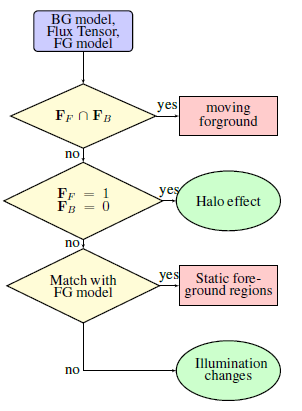
\includegraphics[scale=0.8]{img/FTSG_flow.png}
				\caption{Schemat operacji algorytmu \textit{FTSG}}
				\label{fig:FTSG_flow}
		\end{figure}
		
		\begin{figure}[h]
				\centering
				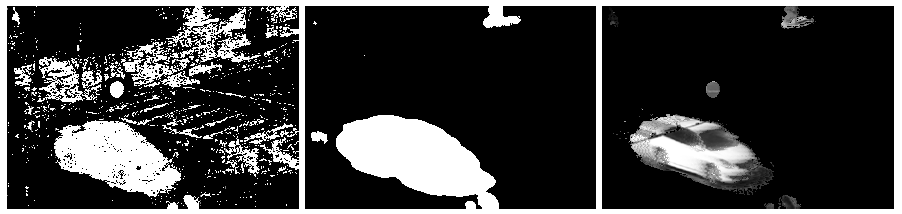
\includegraphics[scale=0.65]{img/ftsg_models.png}
				\caption{Przykładowe maski binarne otrzymane odpowiednio dla modelu tła, metody \textit{Flux Tensor} i modelu pierwszego planu}
				\label{fig:ftsg_models}
		\end{figure}

Jeżeli piksel zostanie przez obie metody tak samo sklasyfikowany, to jego ostateczna przynależność jest oczywista. W takim przypadku piksel zostaje uznany za obiekt ruchomy ($F_F = 1 \land F_B = 1$) bądź statyczne tło ($F_F = 0 \land F_B = 0$). Na rysunku \ref{fig:ftsg_moving_obj} została przedstawiona część wspólna masek binarnych obu modułów oraz zidentyfikowany obiekt. 

Dodatkowa analiza ma miejsce w przypadku, gdy wyniki obu modeli są sprzeczne. Jeżeli metoda \textit{Flux Tensor} oznaczy próbkę jako pierwszy plan, natomiast model tła jako element tła, to końcowym werdyktem jest zaklasyfikowanie piksela jako tło. Jest to logicznie uzasadnione, ponieważ \textit{Flux Tensor} ma tendencję do zaznaczania obiektów o trochę większym obszarze niż są one w rzeczywistości (tzw.~efekt halo). Dodatkowo metoda bazująca na rozkładach Gaussa bez problemu wykrywa obiekty będące w ruchu, zatem takie działanie nie powoduje utraty istotnych danych. Taki przypadek został przestawiony na rys. \ref{fig:ftsg_halo}.

		\begin{figure}[h]
				\centering
				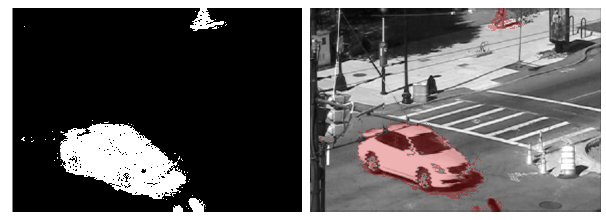
\includegraphics[scale=0.65]{img/ftsg_moving_obj.png}
				\caption{Detekcja ruchomego obiektu}
				\label{fig:ftsg_moving_obj}
		\end{figure}
		
		\begin{figure}[h]
				\centering
				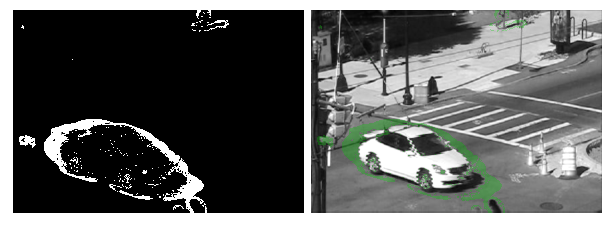
\includegraphics[scale=0.65]{img/ftsg_halo.png}
				\caption{Przykład tzw. efektu halo}
				\label{fig:ftsg_halo}
		\end{figure}

W przypadku odwrotnym, czyli $F_F = 0 \land F_B = 1$, wykorzystywany jest model pierwszoplanowy i na jego podstawie wyznaczane jest ostateczne dopasowanie. Jeżeli dla zdefiniowanego w tym modelu rozkładu Gaussa piksel wejściowy spełnia warunek (\ref{equ:F_S}) to zostaje zakwalifikowany jako element statyczny pierwszego planu ($F_S = 1$). Model pierwszoplanowy jest aktualizowany tylko wtedy, gdy prawdziwy jest warunek $F_F = 0 \land F_B = 1 \land F_S = 1$. W przeciwnym wypadku ma miejsce aktualizacja modelu tła. Przykład detekcji obszaru statycznego został przedstawiony na rys. \ref{fig:ftsg_static}.

		\begin{figure}[h]
				\centering
				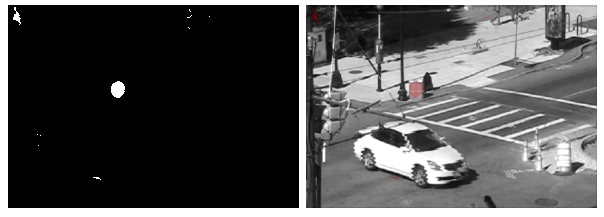
\includegraphics[scale=0.65]{img/ftsg_static_obj.png}
				\caption{Detekcja obszaru statycznego}
				\label{fig:ftsg_static}
		\end{figure}

Taka klasyfikacja pozwala wyeliminować większość szumów powstałych w modelu tła, między innymi na skutek zmian oświetlenia i innych zakłóceń (przykładowe szumy w modelu tła zostały przedstawione na rys. \ref{fig:ftsg_illumination}). Należy przy tym pamiętać, że współczynnik $k$ w podanym wzorze jest inny dla obu modeli. Istotne jest także, że w niektórych przypadkach obiekt statyczny może być w rzeczywistości odsłoniętym tłem przez właśnie ruszający obiekt (np. samochód odjeżdżający z parkingu). Problem ten jest częściowo eliminowany przez zastosowanie różnych stałych uczenia się ($\alpha$) w obu modelach wykorzystujących rozkłady Gaussa.

	    \begin{figure}[h]
				\centering
				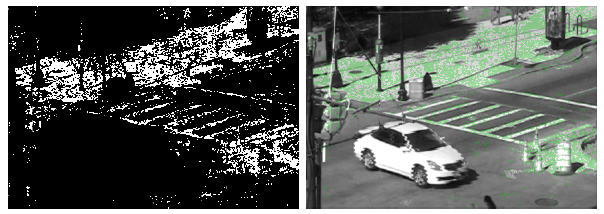
\includegraphics[scale=0.65]{img/ftsg_illumination.png}
				\caption{Szumy powstałe w modelu tła}
				\label{fig:ftsg_illumination}
		\end{figure}

% \section{Detekcja obiektów zatrzymanych}
% \label{sec:detekcja_statyczna}

% W poprzednim podrozdziale zostało wspomniane, że model pierwszego planu klasyfikuje jako obiekt statyczny także obszar odsłoniętego tła. Jest to wspominany wielokrotnie efekt ,,duchów''. Może on zostać częściowo wyeliminowany poprzez dobranie odpowiedniego parametru $\alpha$. Niestety, ze względu na specyfikę metod wykorzystujących rozkłady Gaussa, nie jest możliwa jego całkowita eliminacja. W~tym celu został opracowany dodatkowy mechanizm rozróżniania rzeczywistych obiektów zatrzymanych od odsłoniętego tła. 

% Opisywana metoda wykorzystuje trzy obrazy: wejściowy, model tła oraz maskę binarną otrzymaną z modelu pierwszego planu. Kolejnym krokiem jest wykrycie krawędzi (metodą Sobela) na wszystkich trzech obrazach. Ostatnią czynnością jest porównanie i analiza rezultatów. Jeżeli kształt krawędzi na obrazie wejściowym i wygenerowanym pierwszym planie jest podobny, obiekt może zostać zinterpretowany jako statyczny (tj. zatrzymany obiekt). Natomiast, jeśli krawędzie w modelu tła oraz pierwszego planu są do siebie zbliżone, to wykryty obiekt jest klasyfikowany jako odsłonięte tło. Na rysunkach \ref{stoppedObj} i~\ref{revBg} zostały przedstawione przykłady ilustrujące oba przypadki.

% \begin{figure}[h]
% 	\centering
%     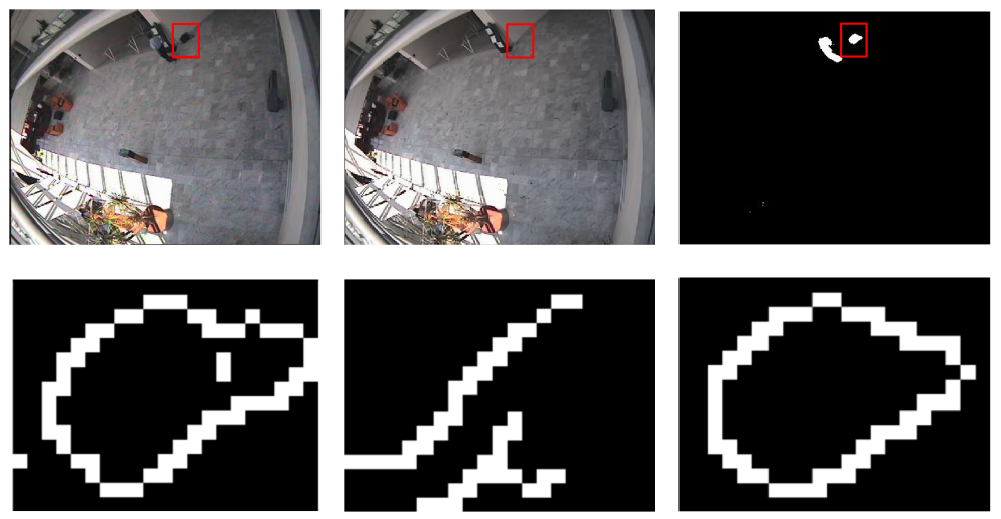
\includegraphics[scale=0.5]{img/stoppedObject.png}
% 		\caption{obiekt zatrzymany}
% 		\label{stoppedObj}
% \end{figure}

% \begin{figure}[h]
% 		\centering
% 		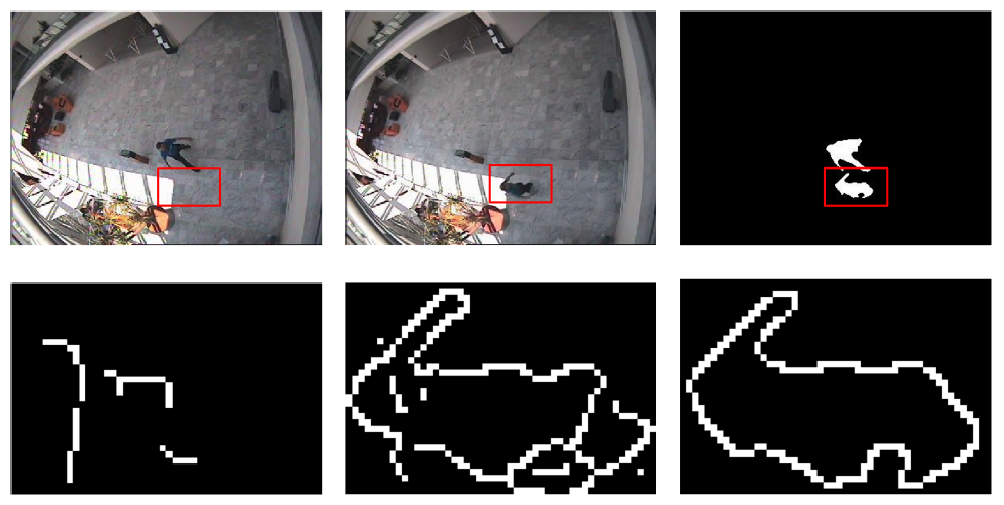
\includegraphics[scale=0.5]{img/revealedBg.png}
% 		\caption{odsłonięte tło}
% 		\label{revBg}
% \end{figure}

% Na rysunku \ref{stoppedObj} umieszczone zostały w pierwszym rzędzie kolejno: obrazek wejściowy, model tła oraz maska otrzymana przez model pierwszoplanowy. W~rzędzie drugim znajdują się obrazy po zastosowaniu detekcji krawędzi. Przedstawiają one zbliżenie na obszar, który został zakwalifikowany jako statyczny przez model pierwszoplanowy i konieczne jest zastosowanie algorytmu detekcji. Jak łatwo zauważyć krawędzie modelu pierwszoplanowego pokrywają się z~krawędziami obrazu wejściowego. Zatem obszar ten jest obiektem statycznym. Rysunek \ref{revBg} przedstawia analogiczną sytuację, jednak w~tym przypadku krawędzie modelu tła i modelu pierwszoplanowego są zbliżone, zatem obszar ten należy interpretować jako odsłonięty fragment tła. Takie działanie pozwala wyeliminować obszary błędnie zakwalifikowane, na podstawie modelu pierwszego planu, jako tło.

\section{Testy}

Ocena jakości procesu segmentacji obiektów pierwszoplanowych ze statycznej kamery jest stosunkowo prosta. Z natury działania algorytmu \textit{FTSG} wynika, że każdy piksel jest klasyfikowany do jednego z dwóch zbiorów: obiektów pierwszoplanowych lub tła. Zatem do oceny działania algorytmu wystarczyło zastosować test binarny. 

Do oceny zastosowano sekwencje testowe ze zbioru dostępnego na stronie \textit{http://www.
changedetection.net/}. Zbiór testowy zawiera również klatki referencyjne
(ang. \textit{ground truth}), które stanowiły punkt odniesienia do oceny algorytmu \textit{FTSG}. Każda z nich była wzorcowym przekształceniem obrazu wejściowego na wyjściowy, na którym kolorem białym wyróżniono obiekty pierwszego planu. Dodatkowo sekwencje testowe należało oceniać od pewnego ustalonego numeru klatki. Dla każdego testu był on inny.

Na podstawie porównania wszystkich ramek wyjściowych testowanej metody oraz odpowiadających im wzorców wyznaczane są następujące wartości (składowe testu klasyfikacji binarnej):
\begin{itemize}
	\item$\small TP$ -- liczba pikseli poprawnie zakwalifikowanych jako pierwszy plan (ang. \textit{true positive})
	\item $\small TN$ -- liczba pikseli poprawnie zakwalifikowanych jako tło (ang. \textit{true negative})
	\item $\small FN$ -- liczba pikseli błędnie zakwalifikowanych jako tło (ang. \textit{false negative})
	\item $\small FP$ -- liczba pikseli błędnie zakwalifikowanych jako pierwszy plan (ang. \textit{false positive})\\
\end{itemize}

\noindent Po obliczeniu wszystkich czterech współczynników dla danej sekwencji wyznacza się 7 wskaźników, które określają dokładność metody:
%
\TabPositions{0.45\linewidth}
\begin{enumerate}%[nolistsep]
	\item \textit{Recall (Re)} : \tab \small{$TP/(TP+FN)$}
	\item \textit{Specificity (Spec)} : \tab \small{$TN/(TN+FP)$}
	\item \textit{False Positive Rate (FPR)} : \tab \small{$FP/(FP + TN)$}
	\item \textit{False Negative Rate (FNR)} : \tab \small{$FN/(FN + TP)$}
	\item \textit{Percentage of Wrong Classifications (PWC)} : \tab \small{$100(FN + FP)/(TP + FN + FP + TN)$}
	\item \textit{Precision (Pr)} : \tab \small{$TP/(TP + FP)$}
	\item \textit{F-measure (F1)} : \tab \small{$2\frac{P_r*R_e}{P_r+R_r}$}\\
\end{enumerate}

Do weryfikacji modelu programowego algorytmu stworzone zostało automatyczne środowisko testowe (w~\textit{Pythonie}). Dla każdego testu wykonywane były następujące czynności:

\begin{itemize}
	\item Podmiana makra w kodzie modelu programowego, definiującego wybraną sekwencje testową (domyślnie wybrana była pierwsza sekwencja testowa).
	\item Ponowna kompilacja modelu programowego.
	\item Uruchomienie modelu programowego dla wybranej sekwencji testowej.
	\item Po zakończeniu testu, zapamiętanie otrzymanych współczynników ze standardowego wyjścia uruchamianego programu (\textit{TP, TN, FP, FN}).

\end{itemize}

\noindent Po przeprowadzeniu testów dla wszystkich sekwencji testowych generowany był raport zawierający współczynniki jakości każdej sekwencji testowej. Dana zapisywane były do pliku. 

Takie podejście znacząco ułatwia testowanie algorytmu \textit{FTSG} z uwagi na jego złożoność obliczeniową. Dla sekwencji testowych w rozdzielczości $320 \times 240$ model programu przetwarza obraz z prędkością około 5 klatek na sekundę. W konsekwencji przetestowanie wszystkich sekwencji trwa około 4 godzin. Stworzone środowisko testowe jest w stanie przeprowadzić cały proces automatycznie bez jakiegokolwiek nadzoru. Dodatkową korzyścią jest prosta weryfikacja wprowadzonych modyfikacji. Środowisko testowe kompleksowo udziela odpowiedzi na pytanie, czy wprowadzona zmiana w algorytmie polepsza albo pogarsza jakość segmentacji obiektów pierwszoplanowych. Poza tym, ręczne testowanie na jednej czy nawet dwóch sekwencjach może być niebezpieczne, gdyż możemy przypadkowo wprowadzić poprawki, które sprawdzają się jedynie dla tej szczególnej sekwencji testowej.

\section{Podział pracy}

Piotr Janus -- algorytm \textit{Flux Tensor}, fuzja metod \textit{FT} i \textit{Split Gaussian Models} (model programowy), analiza artykułu i sformułowanie pytań do autorów, przygotowanie prezentacji i niniejszego raportu.

Kamil Piszczek --  \textit{Split Gaussian Models} (model programowy), zaprojektowanie i implementacja środowiska testowego,  analiza artykułu i sformułowanie pytań do autorów i niniejszego raportu. 

\end{document}
